Let us consider $\triangle PQR $ right angled at $Q$
and assume that we are restricted to first quadrant such that
\begin{align}
\vec{Q} = \myvec{0\\0}, \vec{R} = \myvec{4\\0}, \vec{P} = \myvec{0\\p}
\end{align}
Then,
% \begin{align}
% \norm{\vec{R}-\vec{Q}} = \norm{\vec{R}}  = 4  \quad \brak{\because \vec{Q}=0}
% \end{align}
% This indicates that length of leg QR is 4.
\begin{align}
\norm{\vec{P}-\vec{R}}^2 &= 36
\\
\implies  p^2 + 16 &=36
%\end{align}
% Also hypotenuse is 6,
% \begin{align}
% \implies\norm{{\vec{P}-\vec{R}}}^2=6^2=36
% \end{align}
% Therefore,
% \begin{align}
% p^2 + 16=36
% \\
% \implies p^2=20
 \\
\implies p &=\pm 2\sqrt{5}
\end{align}
Since first quadrant was assumed here,only $p=+2\sqrt{5}$ is taken into consideration.
So,the vertices of $\triangle PQR$ in Fig. \ref{constr/25/fig:right_angle_triangle} are
\begin{align}
\vec{P} = \myvec{0\\2\sqrt{5}}, \vec{Q} = \myvec{0\\0}, \vec{R} = \myvec{4\\0}
\end{align}
% Lines $PQ$ ,$QR$ and $RP$ are then generated and
% plotted using these coordinates to form $\triangle PQR$ .
% Plot of the right angled $\triangle PQR$ is given below:
%
\begin{figure}[!ht]
\centering
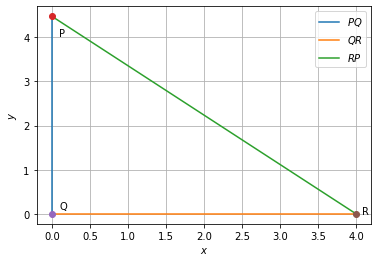
\includegraphics[width=\columnwidth]{solutions/25/Figures/figure1.png}
\caption{ Right Angled $\triangle PQR$}
\label{constr/25/fig:right_angle_triangle}	
\end{figure}
